Lastly, this section presents the final TRITIUM monitor, a schematic design of which is shown in Figure \ref{fig:TritiumDetectorSchematicDesign}.

\begin{figure}[h]
\centering
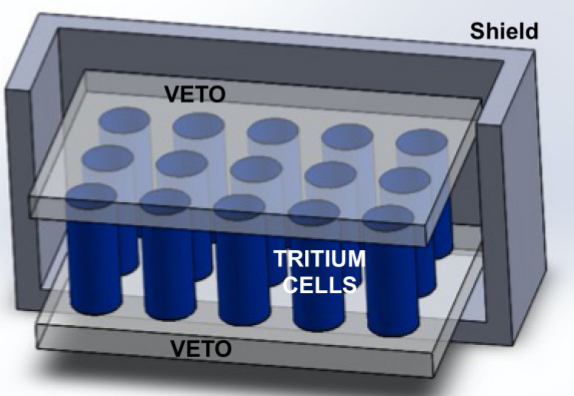
\includegraphics[scale=0.5]{5Prototypes/55ModularTritiumDetector/FinalTritium.png}
\caption{A schematic design of the TRITIUM detector.\label{fig:TritiumDetectorSchematicDesign}}
\end{figure}

It consists of several TRITIUM modules, shown in Figure \ref{fig:TritiumDetectorSchematicDesign}, which are read in parallel. Each module will be the prototypes that achieves better results, TRITIUM-Aveiro 0 (section \ref{subsec:TritiumAveiro}) or TRITIUM-IFIC 2 (section \ref{subsec:TritiumIFIC2}).

These modules are isolated from environmental radioactivity using three different techniques.

\begin{enumerate}

\item{} First, an external lead shielding, explained in section \ref{subsec:SetUpPassiveShield}, a part of which is shown in Figure \ref{fig:TritiumDetectorSchematicDesign}. This is used to stop the environmental radioactivity which increase the radioactive background measurement of the TRITIUM monitor

\item{} Second, several active vetos, expained in section \ref{subsec:SetUpActiveShield} and characterized in section\ref{sec:TritiumActiveVeto}, which is shown in Figure \ref{fig:TritiumDetectorSchematicDesign}, placed below and above the TRITIUM modules. These active vetos are read in anticoincidence to eliminate the effect of the high energy events of the background, mainly cosmic events, on the TRITIUM measurement.

\item{} Finally, the radioactive elements present in the water samples, introduced into TRITIUM modules to be measured, are eliminated using an ultrapure water system, shown in section \ref{sec:UltraPureWaterSystem} and appendix \ref{App:UltraPureWaterSystem} and characterized in section \ref{sec:CharacterizationUltraPureWaterSystem}.

\end{enumerate}

The ultrapure water system, lead shielding and a TRITIUM-Aveiro 0 prototype are installed and currently in operation at the Arrocampo dam. This entire system was used to successfully monitor the tritium levels in Arrocampo dam during three months. Furthermore, two TRITIUM-Aveiro 0 prototypes and and four active vetos are currently under manufacturing to be installed, which are measured in parallel with the current prototype installed.

The RaspberryPi, in which the counter electronic system of TRITIUM-Aveiro prototype is based, has some counting limitations if multiple modules are used. To overcome this problem, it must be replaced with an FPGA-based counter board to ensure reliable counting.

At the same time, three TRITIUM-IFIC 2 prototypes and an active veto have already been built, the installation of which at the Arrocampo dam was delayed due to the coronavirus pandemic restrictions imposed in Spain. They will be installed as soon as possible.

One of the most important points of the TRITIUM detector is its modular design, with which an scalability can be achieved to reach the required sensitivity, $100~\becquerel/\liter$.  If this sensitivity goal is not reached with the three modules that will be installed, we only need to install some additional modules to improve it.

The only scalability restriction is the available space, which is fixed by the lead shield already built and installed (it is also fixed by the available space in the house where the lead shield is installed). Taking into account the currently available space, five different structures designed for TRITIUM-IFIC 2, one of which is shown in Figure \ref{fig:TritiumMonitorIFIC2Design}, can be used, where ten different modules (grey) and an active veto (black) can be accommodated in any of them. 

\begin{figure}[h]
\centering
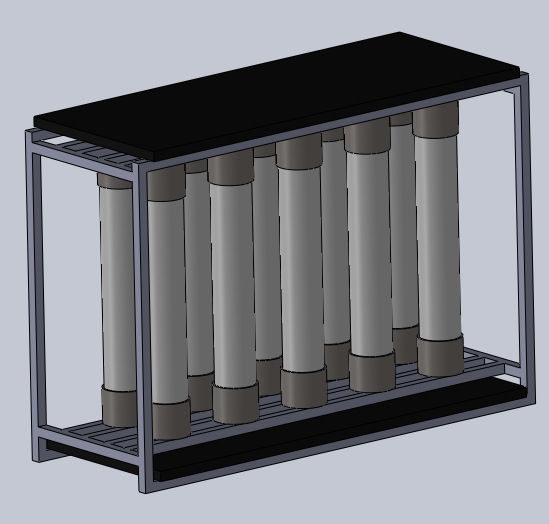
\includegraphics[scale=0.6]{5Prototypes/55ModularTritiumDetector/Tritium_Detector_Based_On_Tritium_IFIC_2.PNG}
\caption{A TRITIUM detector design based on the TRITIUM-IFIC 2 prototype.\label{fig:TritiumMonitorIFIC2Design}}
\end{figure}

It means that up to 50 TRITIUM-IFIC 2 modules can be used in parallel, reducing the TRITIUM detector sensitivity by a factor of fifty. In light of the results obtained with these prototypes, it is not expected to use more than one structure like the one shown in Figure \ref{fig:TritiumMonitorIFIC2Design} (ten modules) to reach the target sensitivity.